%!TEX program = xelatex
%%%%%%%%%%%%%%%%%%%%%%%这是导言部分的开始%%%%%%%%

%========= 导言部分声明文档的类型=================
\documentclass{article}

	%=========导言部分可可以加载宏包=================
	\usepackage{amsmath}                % 数学公式排版宏包
	\usepackage{amssymb}                % 数学符号命令宏包
	\usepackage{amsthm}                 % 数学定理宏包
	\usepackage[UTF8]{ctex}             % 中文输入宏包
	\usepackage[a4paper]{geometry}      % 页面设置宏包
	\usepackage{setspace}               % 行间距宏包
	\usepackage{graphicx}               % 图片宏包
	\usepackage{listings}               % 代码宏包
	\usepackage{color}					% 颜色宏包
	\usepackage{xcolor}                 % 颜色处理宏包
	\usepackage{float}                  % 浮动对象式样宏包
	\usepackage{fontspec}
	
	%=========页面设置==============================
	\geometry{left=1cm,right=1cm,top=1cm,bottom=2cm}
	\onehalfspacing
	\setlength\parindent{0em}

	%=========代码格式设置============================
	\definecolor{dkgreen}{rgb}{0,0.6,0}
	\definecolor{gray}{rgb}{0.5,0.5,0.5}
	\definecolor{mauve}{rgb}{0.58,0,0.82}
	% \setmonofont{Consolas}
	\lstset{
		numbers = left, 	
		numberstyle = \color{gray}, 
		keywordstyle = \color{blue},
		commentstyle = \color{dkgreen}, 
		stringstyle = \color{mauve},
		basicstyle = \ttfamily,
		breaklines = true,
		frame = shadowbox, % 阴影效果
		rulesepcolor = \color{ red!20!green!20!blue!20} ,
		escapeinside = ``, % 英文分号中可写入中文
		xleftmargin = 2em,xrightmargin=2em, aboveskip=1em,
		framexleftmargin = 2em
	} 

%=========导言部分可以定义标题信息===============
\title{组会报告}
\author{徐益}
\date{\today}

%%%%%%%%%%%%%%%%%%%%%%%这是导言部分的结束%%%%%%%%%

%%%%%%%%%%%%%%%%%%%%%%%这是正文部分的开始%%%%%%%%%
\begin{document}
	
%=========生成标题================================
\maketitle

%=========开始正文的输入==========================

%===========第一节=================
\section{本周工作内容}

1. 尝试扩大DPDK的中mbuf

2. 实现分块传输和流量控制问题

3. 处理makefile相关问题

%===========第一节=================
\section{尝试扩大DPDK的中mbuf}
\begin{figure}[H]
	\centering
	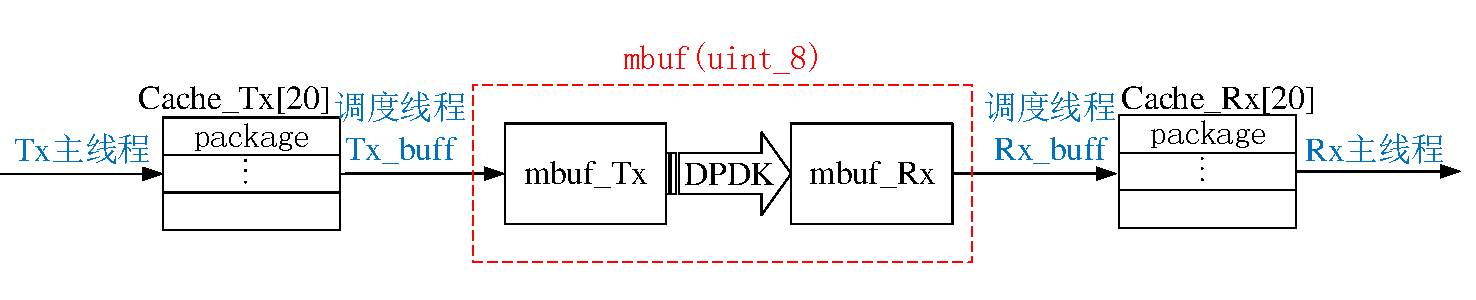
\includegraphics[width = \textwidth]{frame_sys_old.pdf}
	\caption{原系统结构}
\end{figure}
\begin{figure}[H]
	\centering
	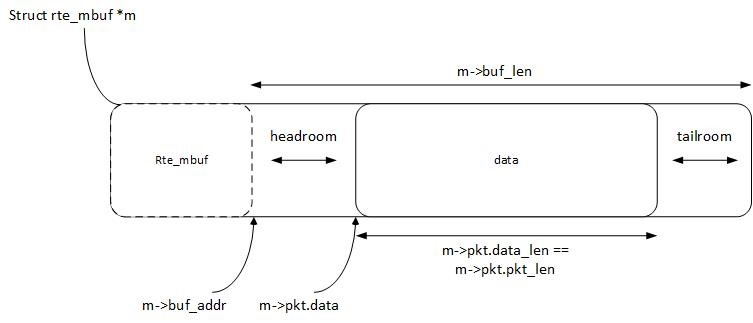
\includegraphics[width = .8\textwidth]{structure_mbuf.jpg}
	\caption{rtl\_mbuf结构}
\end{figure}
\lstset{language=C++}
\begin{lstlisting}
struct rte_mempool *
rte_pktmbuf_pool_create(const char *name, unsigned n,
	unsigned cache_size, uint16_t priv_size, uint16_t data_room_size,
	int socket_id);
\end{lstlisting}
\begin{figure}[H]
	\centering
	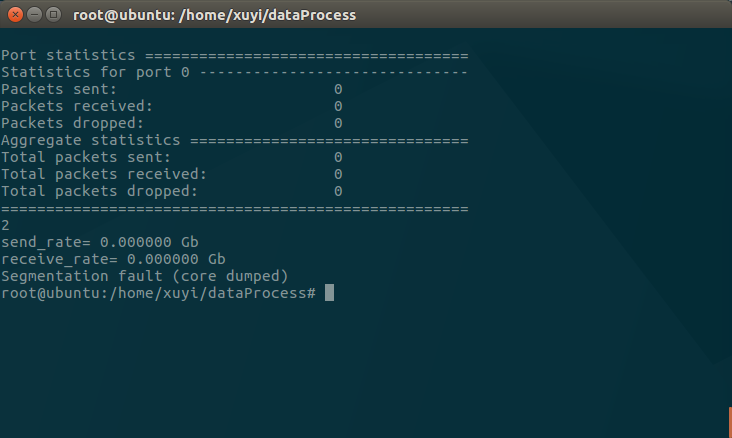
\includegraphics[width = .8\textwidth]{fault_dumped.png}
	\caption{仅扩大MBUF\_SIZE}
\end{figure}
\begin{figure}[H]
	\centering
	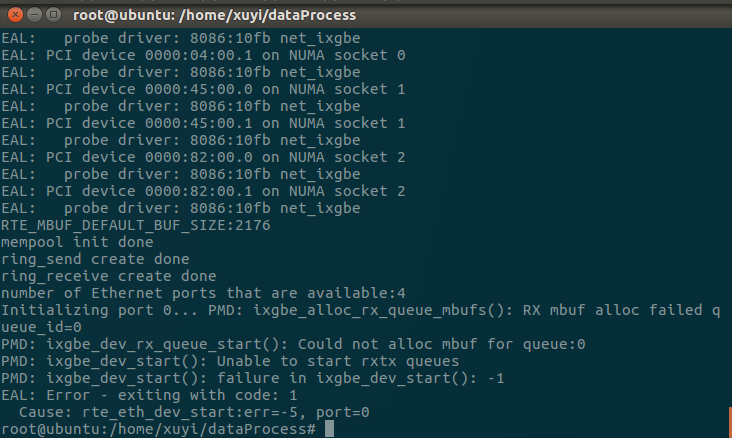
\includegraphics[width = .8\textwidth]{fault_dev.png}
	\caption{扩大MBUF\_SIZE的同时缩小NB\_MBUF}
\end{figure}

%===========第二节=================
\section{分段传输方案}
\begin{figure}[H]
	\centering
	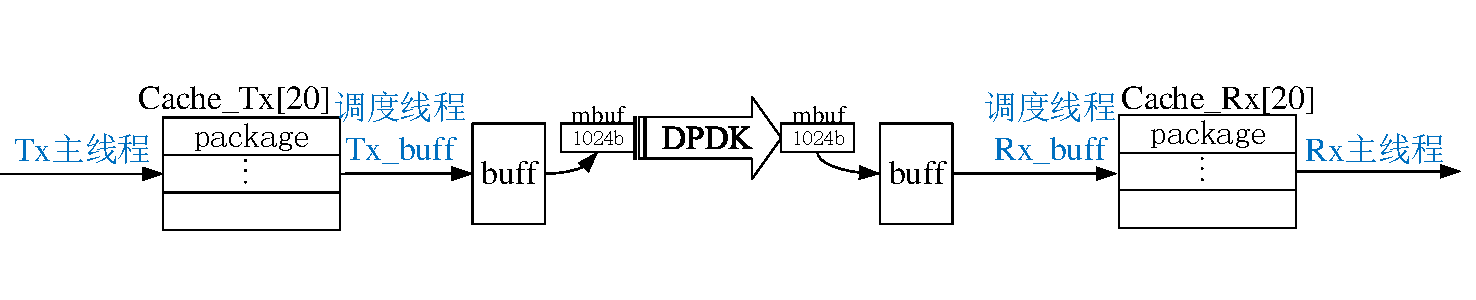
\includegraphics[width = \textwidth]{frame_sys.pdf}
	\caption{分段传输方案系统结构}
\end{figure}
\begin{figure}[H]
	\centering
	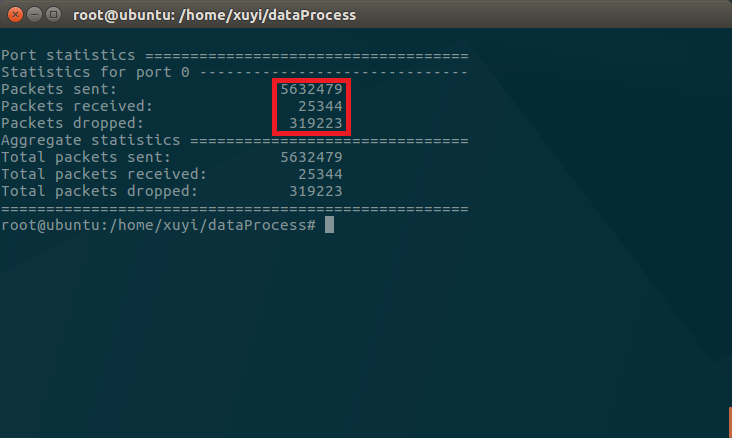
\includegraphics[width = .8\textwidth]{drop_result.png}
	\caption{未进行流量控制}
\end{figure}
\begin{figure}[H]
	\centering
	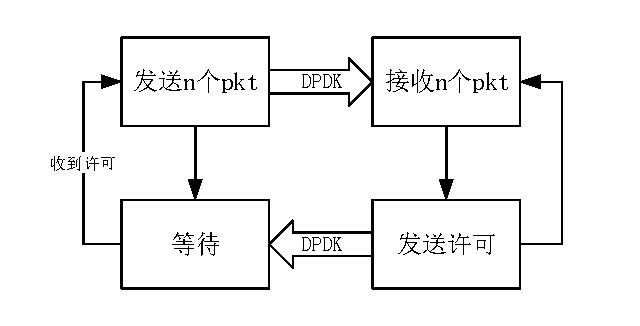
\includegraphics[width = .6\textwidth]{flow_traffic.pdf}
	\caption{流量控制方案}
\end{figure}
\begin{figure}[H]
	\centering
	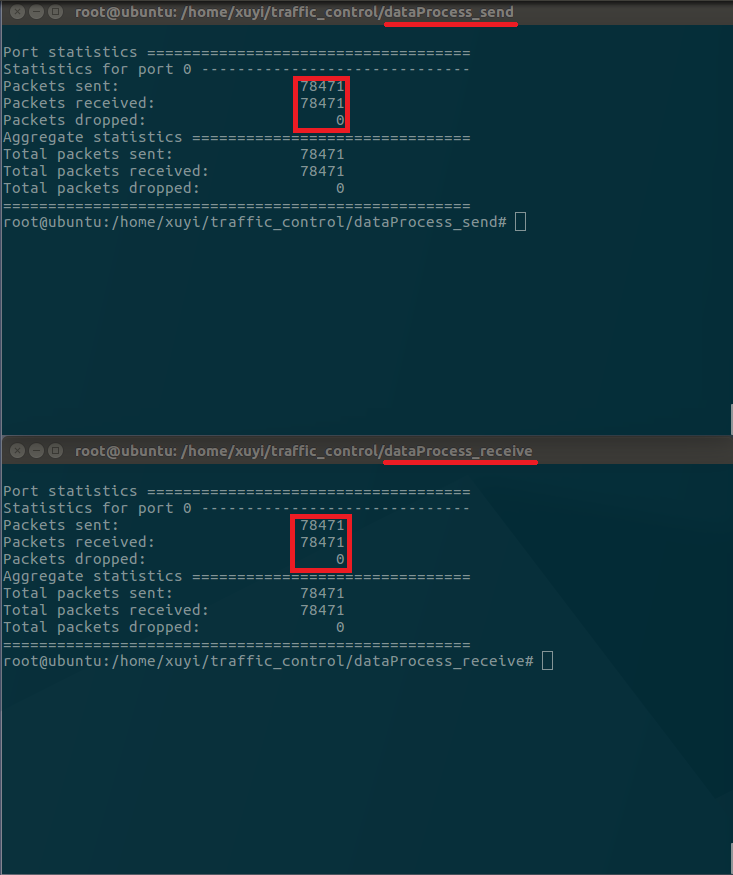
\includegraphics[width = .8\textwidth]{traffic_result.png}
	\caption{进行流量控制后}
\end{figure}

%===========第三节=================
\section{makefile相关问题}
\begin{figure}[H]
	\centering
	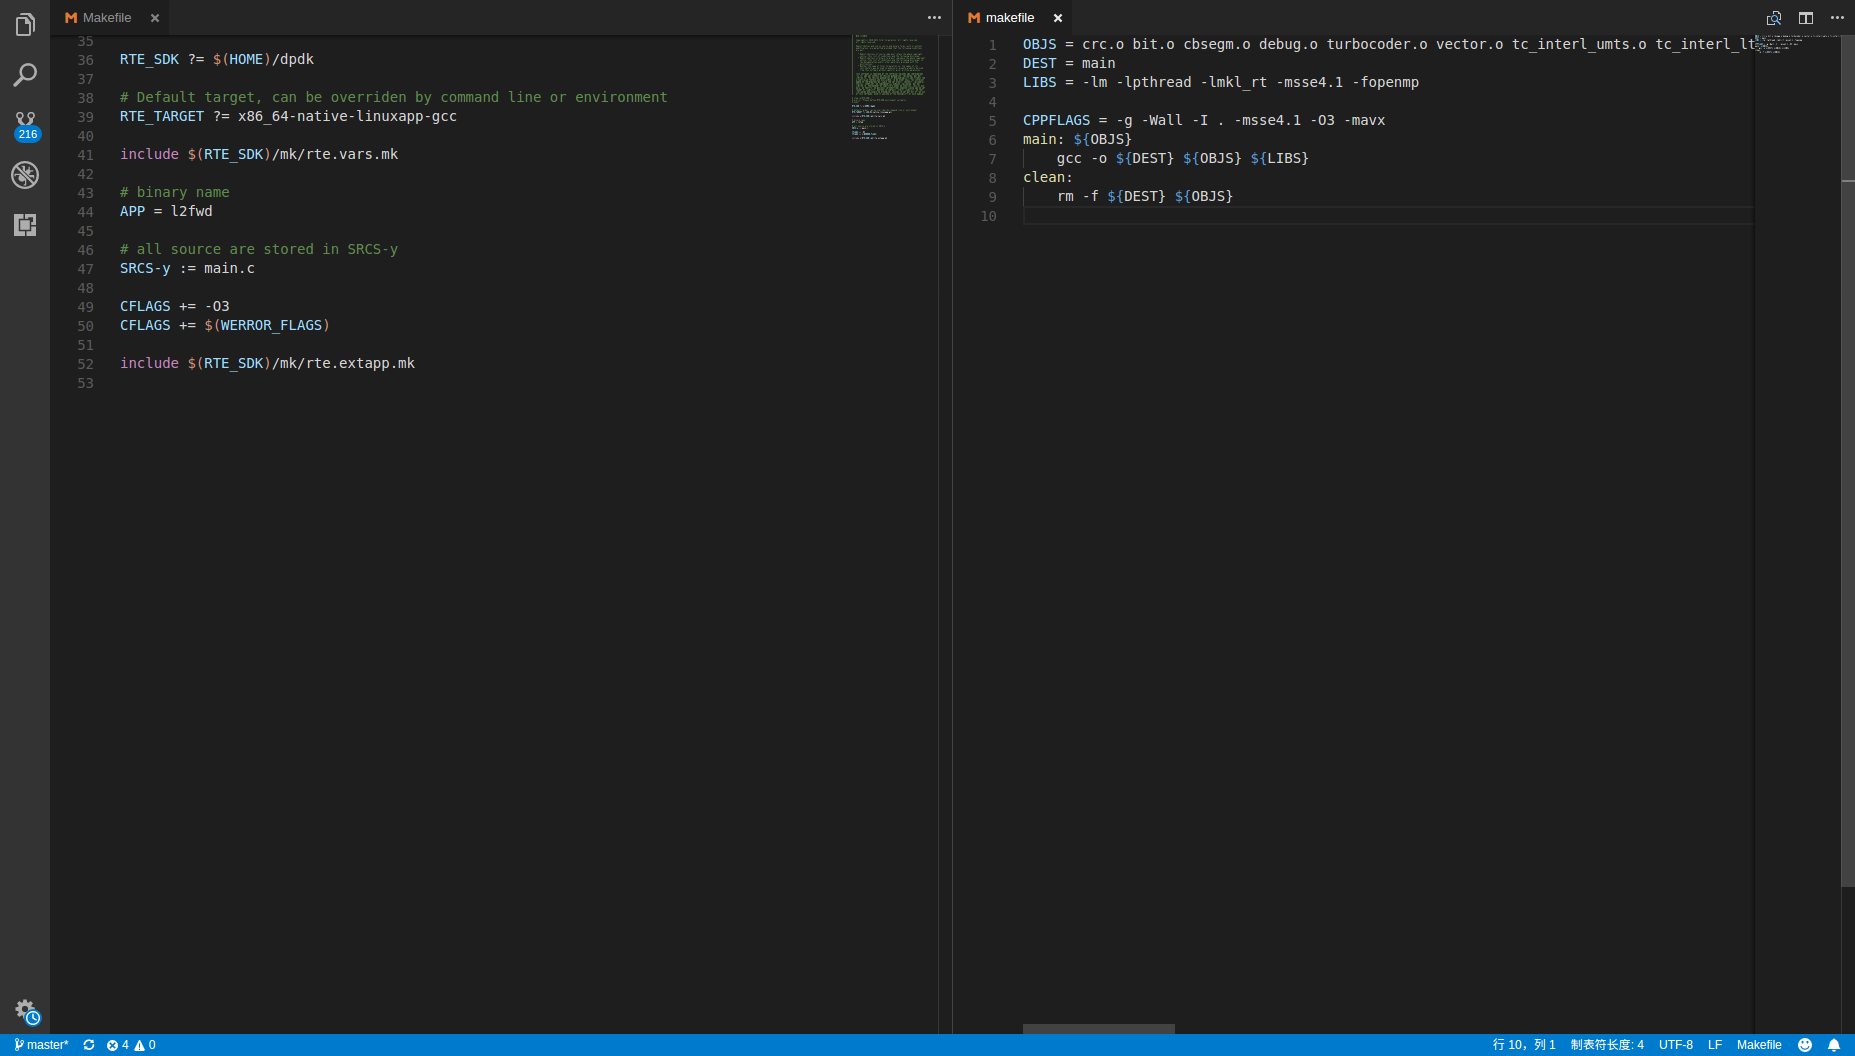
\includegraphics[width = \textwidth]{makefile_compare.png}
	\caption{DPDK和编码调制系统makefile对比}
\end{figure}
\begin{figure}[H]
	\centering
	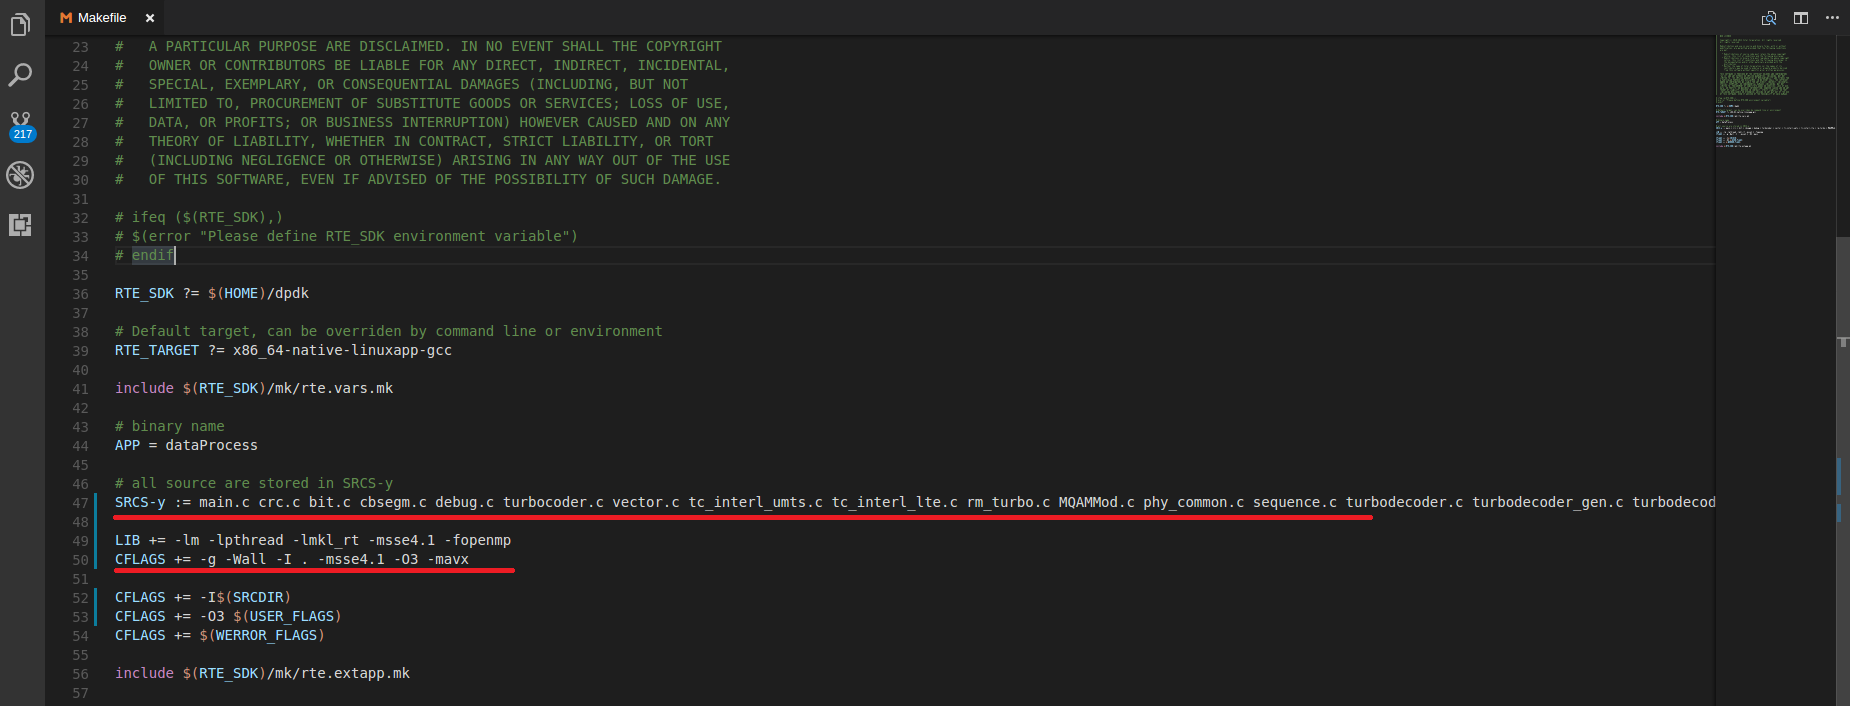
\includegraphics[width = \textwidth]{makefile_try.png}
	\caption{尝试合并的makefile}
\end{figure}
\begin{figure}[H]
	\centering
	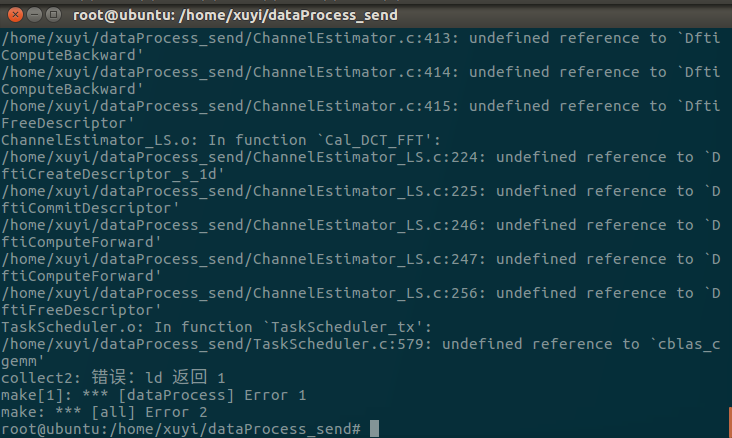
\includegraphics[width = .8\textwidth]{fault_makefile.png}
	\caption{编译报错}
\end{figure}
\begin{figure}[H]
	\centering
	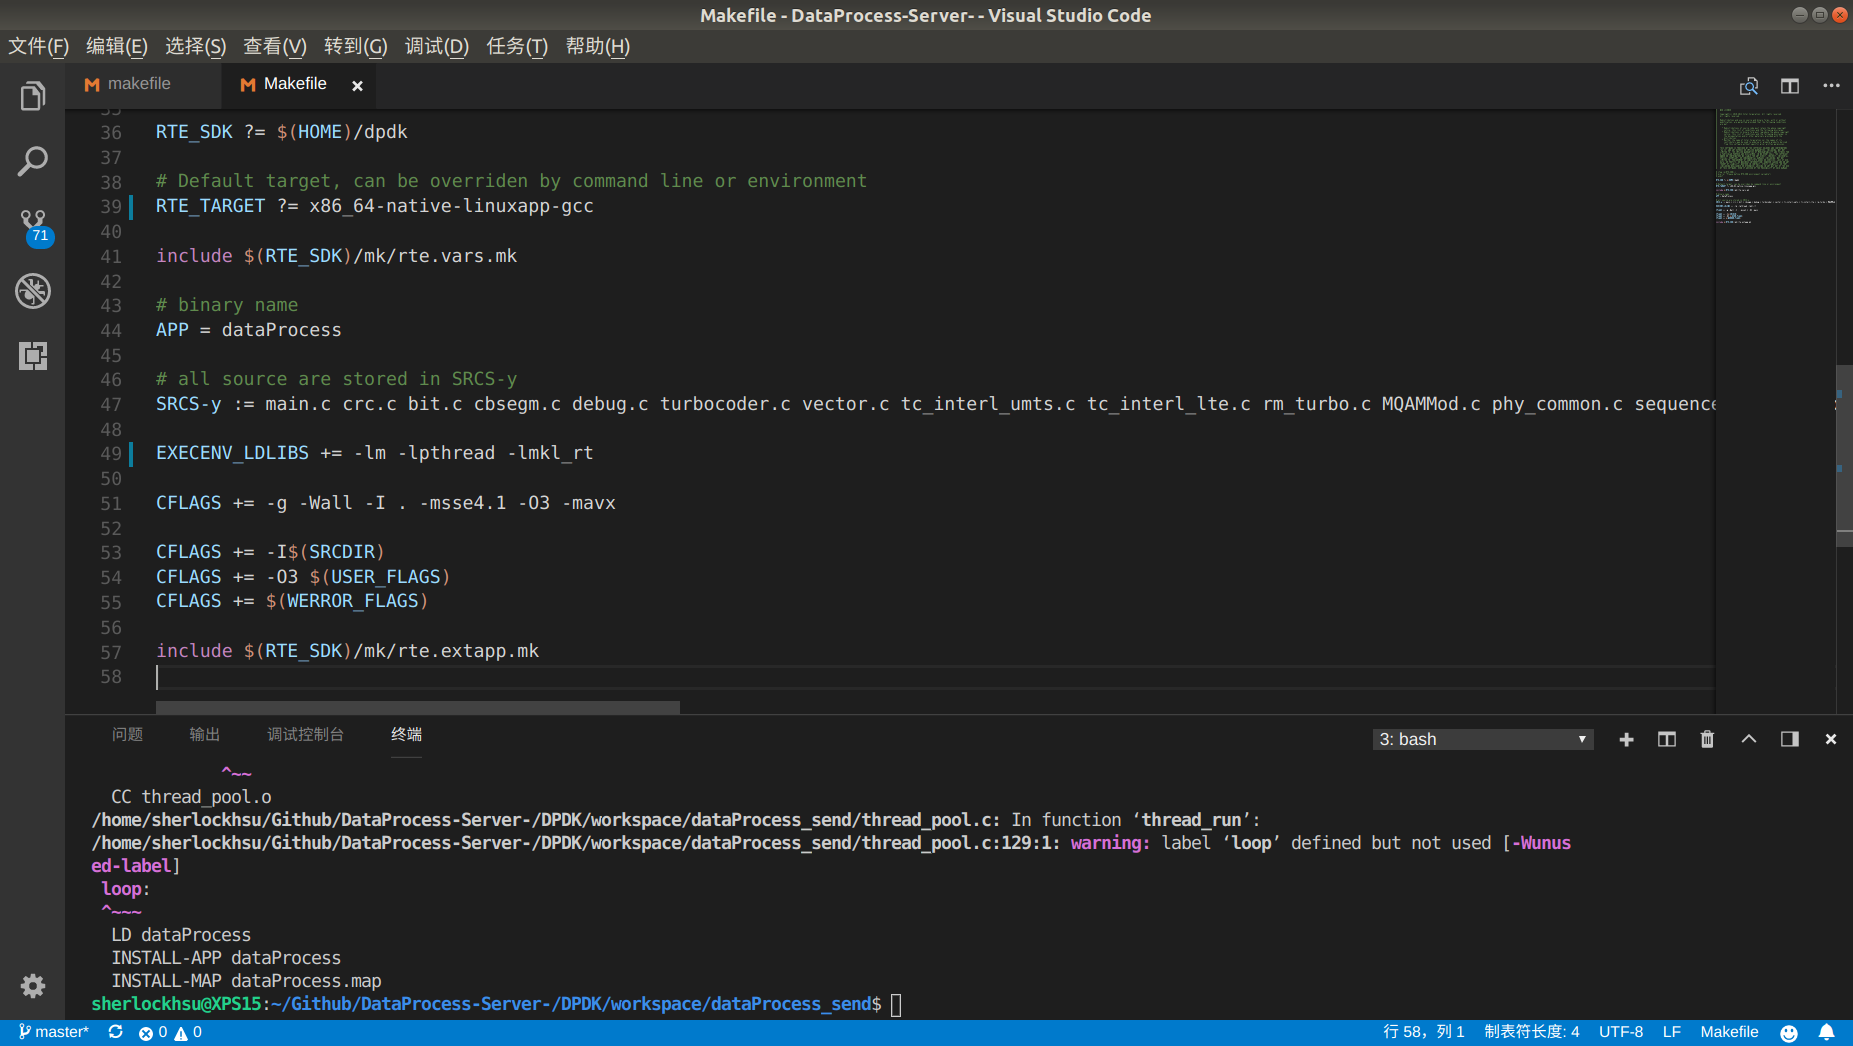
\includegraphics[width = \textwidth]{makefile_final.png}
	\caption{最终解决}
\end{figure}

%===========第四节=================
\section{其他改进方向}
1. 选择更大的DPDK发送页。\\

2. 选择更优的流量控制策略。\\

%===========下周计划=================
\section{下周计划}
1. 继续完成数据处理+DPDK系统

2. 学习LDPC相关内容

\end{document}
%%%%%%%%%%%%%%%%%%%%%%%这是正文部分的结束%%%%%%%%%%%%